\documentclass[]{article}
\usepackage{graphicx}
\usepackage[english]{babel}
\usepackage{standalone}
\usepackage{multicol}
\usepackage[a4paper]{geometry}
\usepackage{enumitem}
\usepackage[normalem]{ulem}
\usepackage{fixltx2e}
\usepackage{color}
\usepackage[hidelinks]{hyperref}
\usepackage{float}
\usepackage{gensymb}
\usepackage{wrapfig}
\usepackage{longtable}
\usepackage{amsmath}
\usepackage[parfill]{parskip}
\usepackage{supertabular,booktabs}
\usepackage{booktabs}
\usepackage{listings}
\usepackage{color}

\definecolor{dkgreen}{rgb}{0,0.6,0}
\definecolor{gray}{rgb}{0.5,0.5,0.5}
\definecolor{mauve}{rgb}{0.58,0,0.82}
\lstset{
  language=Java,
  aboveskip=3mm,
  belowskip=3mm,
  showstringspaces=false,
  columns=flexible,
  basicstyle={\small\ttfamily},
  numbers=none,
  numberstyle=\tiny\color{gray},
  keywordstyle=\color{blue},
  commentstyle=\color{dkgreen},
  stringstyle=\color{mauve},
  breaklines=true,
  breakatwhitespace=true,
  tabsize=3
}
\newcommand{\bftab}{\fontseries{b}\selectfont}



%Paths for graphics locations
\graphicspath{ {./}{../../}{../}{TitlePage/}{Task/}{ExperimentalResults/}}

\begin{document}
	%Insert title page
	\documentclass{article}
\usepackage{graphicx}


\begin{document}

    \begin{center}
    	%title        
        \LARGE
        \textbf{Nature Inspired Optimization}
        
        %subtitle
        \vspace{0.2cm}
        \large
        'Continuous Function Optimisation'
        
        %university logo
        \vspace{1cm}
        
\includegraphics[width=0.9\textwidth]{university}

        \vfill
        
        %team name
        \large
        \textbf{}
        
        %authors
        \vspace{0.3cm}
        \normalsize
        Matthew Flint - 1247903 - mxf203@bham.ac.uk\\
        
		%description
        \vspace{0.5cm}
		This work was conducted as part of the requirements of the Module 06-26949 Nature Inspired Optimisation of the Computer Science department at the University of Birmingham, UK, and is submitted in accordance with the regulations of the University's code of conduct.
		
		%date at end
		\vspace{0.2cm}
		\today
		
		%remove page number
        \pagenumbering{gobble}
    \end{center}
    \newpage
\end{document}
	
	%Insert the abstract
    \pagenumbering{arabic}
    \setcounter{page}{2}
	
	%table of contents
	\newgeometry{bottom=2cm}
	\tableofcontents
	\newpage

	%adjust page width for sections

	\newgeometry{left=1.5cm,right=1.5cm,bottom=2cm,top=1.5cm}
	\documentclass{article}
\usepackage{graphicx}
\usepackage{standalone}
\usepackage{multicol}



\begin{document}
    \section{Introduction}
		This assignment aims to assess how you implement and experimentally compare different nature-inspired
algorithms. It aims at giving you some first hands-on experience of applying a nature-inspired
algorithm in a given context and drawing conclusions about some operators from a set
of experimental results. We consider different mutation operators in the context of continuous
function optimisation.
\end{document}
	\begin{center}
	\hrulefill
	\end{center}
	\documentclass{article}
\usepackage{graphicx}
\usepackage{standalone}
\usepackage{multicol}
\usepackage{amsmath}
\begin{document}
    \section{Task}
    \begin{minipage}{0.5\textwidth}
Consider the following continuous benchmark function SPHERE:
	
$\displaystyle SPHERE(x) = \sum_{i=1}^{n} x_i^2  \text{with}  -\infty < x < \infty$
\\

The SPHERE function has a unique global minimum in:

$\displaystyle SPHERE(x_1,\dotsc,x_n) = SPHERE(0,\dotsc,0) = 0$
\end{minipage}
\begin{minipage}{0.5\textwidth}
    \begin{flushright}
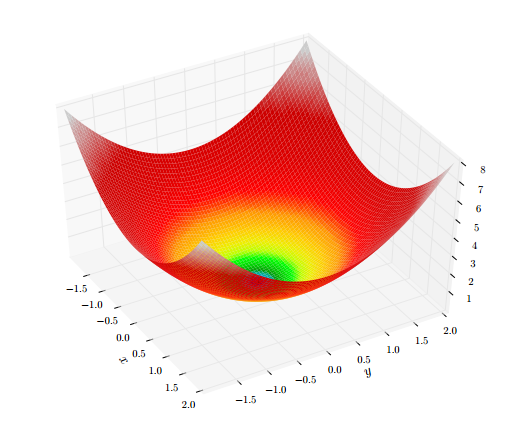
\includegraphics[width=\textwidth]{GraphOriginal}
\end{flushright}
\end{minipage}

and can be visualised for n = 2 as shown above. It is a suitable benchmark to investigate if and
how an algorithm starting from some arbitrary point in the search space is able to converge to a
local optimum, which is an important property for nature-inspired algorithms.
\\

In the lecture you have learned about two mutation operators in the context of continuous function
optimisation, uniform and non-uniform mutation. Here, we consider these and two additional
operators, Gaussian mutation with and without 1/5-rule. You can find explanations and pseudo code
for all four operators in the appendix of this assignment. Your task is to implement and compare
the performance of these four operators on the SPHERE function.
\end{document}
	\begin{center}
	\hrulefill
	\end{center}
	\documentclass{article}
\usepackage{graphicx}
\usepackage{standalone}
\usepackage{multicol}



\begin{document}
    \section{Detailed Instructions}
The assignment requires you to implement the above four operators (Algorithms 2, 3, 4 and 5 in
the appendix) within a simple (1+1) evolution strategy only using mutation (see Algorithm 1 in
the appendix) on the SPHERE function in a programming language of your choice (e. g., Java, C,
C++, Matlab). You will then run a set of experiments as detailed below to assess the performance
of the mutation operators.
Additionally, you are required to describe and discuss your implementation and your experimental
findings in a report. The report should in particular discuss the following aspects (amongst any
other points which you might consider important):

\begin{itemize}

  \item How did you implement the algorithm and the fitness function (e. g., programming language,
design decisions, . . . )? What data structures, algorithms or libraries did you use, e. g., for
a random number generator? What other software/scripts did you use to facilitate your
experiments/analysis?
  \item How does the performance of the different operators compare? How do parameters of the
operators/the fitness function influence the performance?
  \item Try to explain why the operators behave the way you observe in your experiments. What
properties, strengths or weaknesses can you observe? Can you name reasons for them?

\end{itemize}

As a minimum you need to run experiments using the following parameter settings. You are free
to test additional settings if you feel these will help you with the discussion. Make sure to include
these in your report as well. Note that uniform mutation does not have any parameters.

\begin{itemize}
	\item A 10-dimensional SPHERE function (i. e., n = 10) with search space restricted to $[-100, 100]^{10}$
	\item Non-uniform mutation with parameter $b \in \{0.05, 1.0, 10.0, 20.0\}$.
	\item Gaussian mutation without 1/5-rule and parameter $\sigma \in \{0.05, 0.5, 1.0, 10.0\}$
	\item Gaussian mutation with 1/5-rule and initial σ uniformly distributed over [1, 100].
\end{itemize}

You need to perform 30 independent runs for each of the above settings. Each run should have an
upper limit of 5,000 iterations. For each of the runs you need to record the fitness value for each
iteration of the run. Visualise and present your data as follows:

\begin{itemize}
	\item Plot the average function value over time (i. e., iteration number on the x axis; average function
value over the 30 trails on the y axis). Use logscale for the y axes to improve visibility. You
should have such a graph for each of the following scenarios:
	\begin{itemize}
		\item a figure comparing different parameters for non-uniform mutation
		\item a figure comparing different parameters for Gaussian mutation without 1/5 rule
		\item a figure comparing uniform mutation, Gaussian mutation with 1/5 rule and the ‘best’
(i. e., best fitness value after 5,000 iterations) parameter setting for non-uniform and
Gaussian mutation without 1/5 rule
	\end{itemize}
	
	\item Create a table stating the average fitness value and its standard deviation (over the 30 runs)
after 5,000 iterations for each of the considered settings. You can determine these values
with a statistics or spreadsheet software of your choice (e. g., R, Matlab, Microsoft Excel,
LibreOffice).

\end{itemize}

\end{document}
	\begin{center}
	\hrulefill
	\end{center}
	\documentclass{article}
\usepackage{graphicx}
\usepackage{standalone}
\usepackage{multicol}
\usepackage{amsmath}
\usepackage{Listings}
\usepackage{color}

\definecolor{dkgreen}{rgb}{0,0.6,0}
\definecolor{gray}{rgb}{0.5,0.5,0.5}
\definecolor{mauve}{rgb}{0.58,0,0.82}
\lstset{
  language=Java,
  aboveskip=3mm,
  belowskip=3mm,
  showstringspaces=false,
  columns=flexible,
  basicstyle={\small\ttfamily},
  numbers=none,
  numberstyle=\tiny\color{gray},
  keywordstyle=\color{blue},
  commentstyle=\color{dkgreen},
  stringstyle=\color{mauve},
  breaklines=true,
  breakatwhitespace=true,
  tabsize=3
}

\begin{document}
    \section{Implementation}
    I chose to use JAVA as the programming language that I used to implement the algorithms, mainly because it is the language which I have most experience in. This enabled me to quickly convert the pseudo code functions and mathematical equations provided in the assignment JAVA for testing on my machine.\\
    
    \subsection{(1+1) evolution strategy algorithm}
    My implementation allows the user to first choose which mutation algorithm they wish to use via console input out of the four implemented. It then creates the initial search pool for the run, $x = (x_1,\dotsc, x_n)$ by picking $x_i$  uniformly at random from $[-100, 100]$. It then calls a function, iterate(), which loops $T$ times (in my testing this was 5000) calling the selected mutation algorithm for each iteration and storing that iterations fitness calculation into an array. Finally, it outputs the array of the fitness for each iteration to a file. This whole process is then repeated 30 times for the 30 runs of the program we are required to perform and all of the results for each iteration of each run is stored in the output file (with spaces separating each result).\\
    
    This has the effect of the program running and exporting the data for all 30 runs of 5000 iterations in one go which saves a lot of time and allows the data to be exported straight into a spreadsheet application (Excel).\\
    
    \subsection{Fitness Function}
    $\displaystyle SPHERE(x) = \sum_{i=1}^{n} x_i^2  \text{with}  -\infty < x < \infty$
    I implemented the fitness function in a dedicated method inside my code. It has a parameter $X$ which is an array of doubles, which the function calculates the sum of all of the elements squared.
    \begin{lstlisting}
    private double calculateFitness(double[] x) {
		double sum = 0;
		int count = n - 1;
		while (count >= 0) {
			sum = sum + (x[count] * x[count]);
			count--;
		}
		return sum;
	}
    \end{lstlisting}
    I have checked this function against the graph provided for $X[n]$ where $n=2$ which proved successful. Therefore I am confident in my implementation of this method.
    
    \subsection{Fitness Checking}
    I also implemented the method to check the fitness to see if the offspring is better than the parent in its own function. This method first calculates the fitness of the parent \& offspring and then compares them to see which is better. If the offspring is better then the function returns boolean True and if not it returns False.
    \begin{lstlisting}
    private boolean fitnessCheck(double[] offspring) 	{
		// Calculate the fitness of both offspring and X
		double offspringFitness = calculateFitness(offspring);
		double parentFitness = calculateFitness(X);

		// Check which is the better fitness
		if (offspringFitness < parentFitness) {
			return true;
		} else {
			return false;
		}
	}
    \end{lstlisting}
    
    \subsection{Initial search point}
    My function for creating the initial search pool uses Java's Math.random() to generate uniform random numbers to be used as the initial values for the array $X$. I have included a range on the random values produced to that it satisfies $[-100 < X_i < 100]$.
    \begin{lstlisting}
    private void createInitialSearchPool() {
		// Populate the X array with random numbers
		for (int i = 0; i < n; i++) {
			double rand = searchSpaceMin + Math.random() * (searchSpaceMax);
			X[i] = rand;
		}
		System.out.print("Initial value of 'X' set to [ ");
		for (int i = 0; i < n; i++) {
			System.out.print(X[i] + " ");
		}
		System.out.println("]");
	}
	\end{lstlisting}
	
	\subsection{Output File}
	My function to write the output results to a file uses Java's FileReader \& FileWriter functions. It first tries to see if the file already exists and if so it reads it into an array of lines. These lines are then used as prefixes to the current iterations data so that the eventual file contains all 5000 iteration's fitness calculations for each of the 30 runs (results separated by spaces). This data can then be easily parsed into a spreadsheet application.
	
	\subsection{Uniform Mutation Algorithm}
	My implementation of the Uniform Mutation Algorithm uses randomly generated numbers to pick an index of the $X$ array and then replace it with a new value which is also randomly generated (within the bounds of $[-100 < x < 100]$).
	\begin{lstlisting}
	public static double[] UniformMutation(double[] x) {
		double[] xNew = x.clone();

		// pick a random index to mutate
		int max = x.length - 1;
		int min = 0;
		Random rand = new Random();
		int index = rand.nextInt((max - min) + 1) + min;

		// Generate a new random number for that index
		xNew[index] = -10 + Math.random() * (10 - -10);

		return xNew;
	}
	\end{lstlisting}
    
   	\subsection{Non-Uniform Mutation Algorithm}
	My implementation of a non-uniform mutation algorithm chooses a random index of $X$ and then mutates this value by adding or subtracting a random value.The mutation strength, i. e., the size of this change, decreases over time.\\
	
	This implements the algorithm:
	$\bigtriangleup(t,y) = y \cdot {1 - r^{ 1 - {t \over T} }})^b$
	which decreases the size of the mutation change as the number of iterations, $t$, increases. In my code this is also a separate function called NonUniformMutationDelta().
	
	\begin{lstlisting}
	public static double[] NonUniformMutation(double[] x,
			int currentIterationNumber, int numberOfIterations, double b) {
		double[] xNew = x.clone();

		// pick a random index to mutate
		int max = x.length - 1;
		int min = 0;
		Random rand = new Random();
		int index = rand.nextInt((max - min) + 1) + min;
		double newValue;

		// randomly select a mutation
		if (rand.nextDouble() >= 0.5) {
			double nonUniformMutationDelta = NonUniformMutationDelta(
					currentIterationNumber, (100 - xNew[index]), b,
					numberOfIterations);
			newValue = xNew[index] + nonUniformMutationDelta;
		} else {
			double nonUniformMutationDelta = NonUniformMutationDelta(
					currentIterationNumber, (xNew[index] + 100), b,
					numberOfIterations);
			newValue = xNew[index] - nonUniformMutationDelta;
		}
		xNew[index] = newValue;

		return xNew;
	}
	\end{lstlisting}
   	
   	\subsection{Gaussian Mutation}
   	Gaussian mutation adds a normally-distributed random value to each component of the search point. The ‘size’ of this value is controlled by a parameter $\sigma$, which is usually called step size. I used the apache distribution library to generate a normal distribution with standard deviation of 1 and then applied the distribution * step size to each element in the $X$ array.
   	\begin{lstlisting}
   	public static double[] GaussianMutation(double[] x, double stepSize) {
		double[] xNew = x.clone();

		NormalDistribution dist = new NormalDistribution(0, 1);

		for (int i = 0; i < xNew.length; i++) {
			double t = dist.sample();
			xNew[i] = xNew[i] + (stepSize * t);
		}

		return xNew;
	}
   	\end{lstlisting}
   	
   	\subsection{ (1+1) evolution strategy with 1 5-rule}
   	This evolutionary algorithm changes the step size based on how well the algorithm is doing according to the fitness function. It keeps a track of the number of successful \& unsuccessful iterations and adjusts the step size accordingly (If this is larger than 1  5  we double $\sigma$ , if it is smaller $\sigma$ is halved).\\

   	This algorithm uses the Gaussuan mutation as described in the previous section and the changes are implemented in the $(1+1)$ evolution function. Essentially, if the success rate of the evolutions after $i$ iterations is $> 0.2$ then the step size is doubled, else if it is $< 0.2$ then it is halved. This has the effect of broadening \& narrowing possible mutation space for each iteration based on whether the algorithm is a long was off the local optimum.

	\subsection{Software}
	I have used the Eclipse IDE to program the assignment in JAVA, Microsoft Excel has been used as a spreadsheet application to process the data and produces graphs of the results. I have also uses \LaTeX to write \& produce the report.
\end{document}
	\begin{center}
	\hrulefill
	\end{center}
	\documentclass{article}
\usepackage{graphicx}
\usepackage{standalone}
\usepackage{multicol}



\begin{document}
    \section{Experimental Results}
     For all of my testing and the results presented I used a 10-dimensional SPHERE function (i.e. $n=10$) with the search space restricted to $[-100,100]^{10}$.

	\subsection{Non-Uniform Mutation with parameter $b \in \{0.05, 1.0, 10.0, 20.0 \} $}
	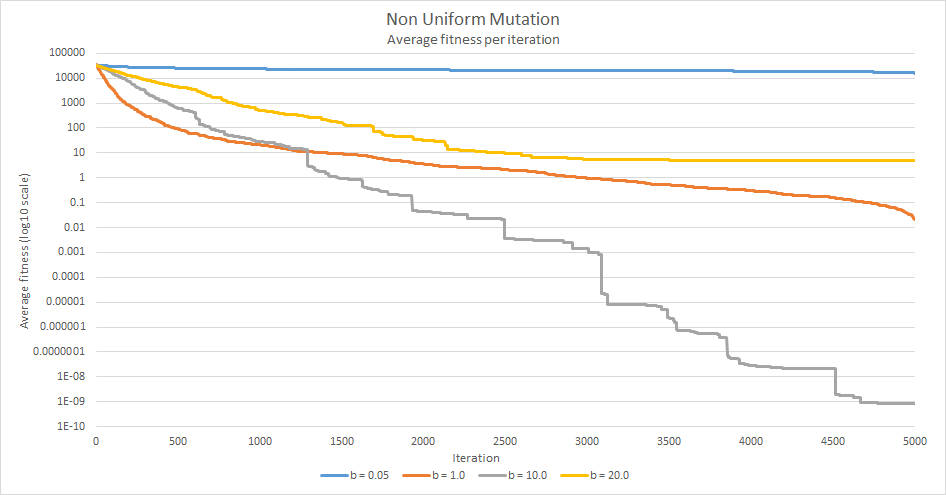
\includegraphics[width=1\textwidth]{Images/NonUniformMutation}\\
	
	As we can see from the graph, for a 10-dimensional sphere function over 5000 iterations the Non-Uniform mutation algorithm did not succeed in finding an optimal solution. The best fitness would have been $0$ but the algorithm does not manage to reach that.\\
	
	The different parameters for $b$ did yield separate and very different results (as shown in the graph). A value of $b=0.05$ produces a very shallow curve with very little reduction in the average fitness value over the 5000 iterations. This proved to be the worst out of all of the parameter values that I tried. This could be due to the way in which the $\Delta(t, y)$ works as the whole second half of the equations is to the exponent $b$. In this case $b=0.05$ which causes the whole equation to become very small, which is then multiplied to the value $y$. This causes a very small overall change in the values of $X$ which could mean that it does not have sufficient time (in the 5000) iterations to deviate very much from its original values.\\
	
	A value of $b=1.0$ produces a rapid initial change (over the first few hundred iterations) which then steadily continues along a constant gradient. The change in the average fitness is greater than with $b=0.05$ and it does get closer to the best average fitness value (with the lowest reached being $0.02$. I believe this is again due to the $\Delta(t, y)$ function as the exponent in this case is $1$ so it is effectively irrelevant. This means that the mutation is directly dependent upon the random number generated for $r$ and the iteration out of the total iterations. This is why it starts to level off after a while, because as $t$ approaches $T$ the value of $r$ approaches $1$ so $\Delta(t, y)$ starts to approach $y \times 1$. This has the effect of not introducing as much variation into each iteration as it would have done at the start of the run.\\
	
	A value of $b=10.0$ produces a constantly declining line which has large jumps in some sections followed by a mini plateau for a while. This value turns out to be the best in my testing as it produced the lowest fitness values out of all of the runs (though it did not achieve the optimal solution). I believe this to be happening because in the $\Delta(t, y)$ equation, $b$ is the exponent, so with this being 10 it is possible to jump large distances between values for $x_i$. However it is not too large so that the value it produces for $x_i$ is either above or below the range $[-100, 100]$ and so would be truncated at the maximum/minimum values. This allows it to gradually step down from its local value.\\
	
	A value of $b=20.0$ produced a very high line on the graph. Is is a worse solution than both $b=1.0$ \& $b=10.0$ however it is better than $b=0.05$. I believe this is due to the $\Delta(t, y)$ equation, $b$ is the exponent, so with this being 20 it is possible to jump large distances between values for $x_i$. In the majority of cases this might push it over the threshold range $[-100, 100]$ which would cause it to be set to the maximum/minimum value. As there is a 50\% chance that either of these cases can happen, and as the value is hitting max/min thresholds often the line tends to stagnate and not vary as much as it could do. This causes it to not seek as many solutions and limits its reach for the best fitness value.\\
	
	From all of this testing I believe that their is a trend that can be seen from the data. \\
	\begin{center}
	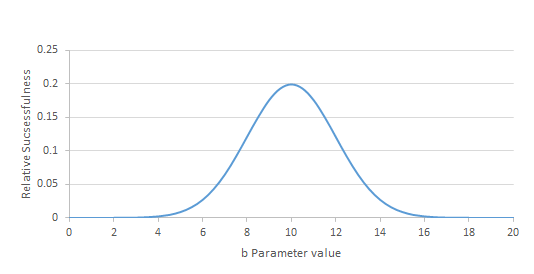
\includegraphics[width=0.8\textwidth]{Images/NonUniformMutationBellCurve}
	\end{center}
	This graph shows the relative successfulness of the algorithm against its $b$ parameter. I would expect that a $b$ value around $10$ to produce the best results and as you go either side of this you start to produce a worse solution.
	
	\subsection{Gaussian mutation without 1/5-rule and parameter $\sigma \in \{0.05, 0.5, 1.0, 10.0\}$}
	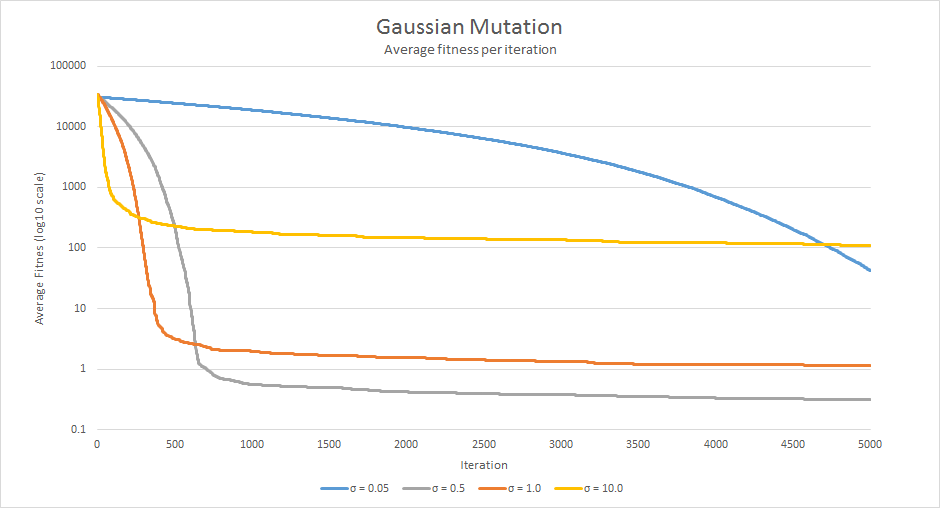
\includegraphics[width=1\textwidth]{Images/GaussianMutation}\\
	
    As we can see from the graph, for a 10-dimensional sphere function over 5000 iterations the Gaussian mutation algorithm did not succeed in finding an optimal solution. The best fitness would have been $0$ but the algorithm does not manage to reach that.\\
	
	The different parameters for $\sigma$ did yield separate and very different results (as shown in the graph). A value of $\sigma=0.05$ produces a very shallow curve (comparably) with a gradual reduction in the average fitness as the iterations continue. This is likely to be because $\sigma$ is very small so the equation $x_i = x_i + \sigma \times m_i$ will have a very small quantity added to it, so it will not vary very much.\\
	
	A value of $\sigma=0.5$ produces better results, a very steep drop over the first few hundred iterations followed by a plateau of very little change. This produced the best result as it achieved the lowest average fitness value.\\
	
	A value of $\sigma=1.0$ produces similar results to $\sigma=0.5$, a very steep drop over the first few hundred iterations followed by a plateau of very little change. However it did not find a fitness value quite as low and was about $3\times$ worse.\\
	
	Finally, a value of $\sigma=10.0$ produces a very steep initial search over just a couple of hundred iterations. However it soon levels out and then there is not much change for the remainder of the 5000 iterations.
	
	\subsection{Comparison of Uniform Mutation, Gaussian mutation with 1/5 rule and the ‘best’ parameter setting for non-uniform and Gaussian mutation without 1/5 rule.}
	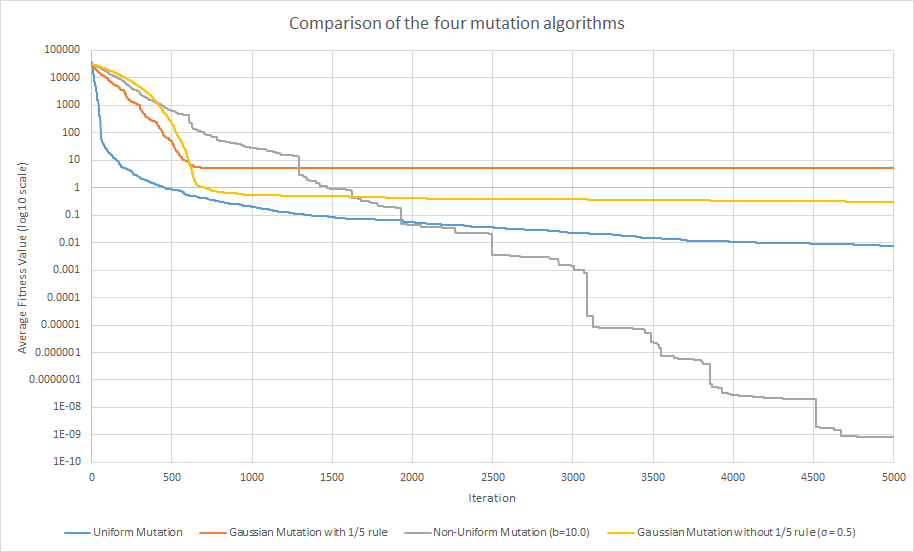
\includegraphics[width=1\textwidth]{Images/ComparisonOfAlgorithms}\\
	
	This comparison graph of all of the four different mutation algorithms (choosing the best parameters in the case of Non-Uniform and Gaussian mutation without 1/5 rule) shows clearly that one of the algorithms far surpasses the others in terms of finding the best fitness value. That is the Non-Uniform mutation algorithms with a parameter of $b=10.0$.\\
	
	We can also see how the others compare to each other, with Uniform Mutation coming in 2\textsuperscript{nd} (though far behind 1\textsuperscript{st} place). 3\textsuperscript{rd} going to Gaussian Mutation without 1/5 rule and a parameter of $\sigma=0.5$. And finally Gaussian Mutation with 1/5 rule coming in last.
	
	
	
\end{document}
	\begin{center}
	\hrulefill
	\end{center}
	\documentclass{article}
\usepackage{enumitem}
\usepackage{gensymb}
\usepackage[normalem]{ulem}
\usepackage{fixltx2e}
\usepackage{color}
\usepackage[hidelinks]{hyperref}
\usepackage{graphicx}
\usepackage[top=2cm,bottom=2cm,left=3cm,right=3cm]{geometry}
\usepackage{multicol}
\usepackage{float}
\usepackage{wrapfig}
\usepackage{longtable}



\begin{document}
\section{Appendix}
A copy of the spreadsheet used to collate the data from the various runs is available \href{https://github.com/Mattie432/Nature-Inspired-Optimization/blob/master/Report/Assignment1/Spreadsheet.xlsx}{\textcolor{blue}{\uline{here}}}.\\
A viewable version of the project code (JAVA) is available \href{https://github.com/Mattie432/Nature-Inspired-Optimizationx}{\textcolor{blue}{\uline{here}}}.

\section{References}
\begin{enumerate}
\item Theprojectspot.com. Creating a genetic algorithm for beginners. 2015.\\ Available at: \href{http://www.theprojectspot.com/tutorial-post/creating-a-genetic-algorithm-for-beginners/3}{\textcolor{blue}{\uline{www.theprojectspot.com/tutorial-post/creating-a-genetic-algorithm-for-beginners/3}}}\\ Accessed February 21, 2015.

\item HERRERA F, LOZANO M. Two-Loop Real-Coded Genetic Algorithms With Adaptive Control Of Mutation Step Sizes.; 2000. \\Available at: \href{http://sci2s.ugr.es/publications/ficheros/ApInt-13(3)-187-204.pdf}{\textcolor{blue}{\uline{sci2s.ugr.es/publications/ficheros/ApInt-13(3)-187-204.pdf}}}\\ Accessed February 23, 2015.

\item Zhao X, Gao X. Evolutionary Programming Based On Non-Uniform Mutation.; 2004. \\Available at: \href{http://mmrc.iss.ac.cn/mm/mm23/MMpreprint\%E8\%B5\%B5\%E6\%96\%B0\%E8\%B6\%85.pdf}{\textcolor{blue}{\uline{mmrc.iss.ac.cn/mm/mm23/MMpreprint\%E8\%B5\%B5\%E6\%96\%B0\%E8\%B6\%85.pdf}}}\\Accessed February 24, 2015.

\end{enumerate}
\end{document}
	\begin{center}
	\hrulefill
	\end{center}
\end{document}
